\section{Quadriken}

Sei $n\in\natur$.

\begin{definition}[Quadrik]
	\proplbl{6_8_1}
	Eine \begriff{Quadrik} ist eine Teilmenge von $\real^n$ mit
	\begin{align}
		Q=\{x\in\real^n\mid x^tAx+2b^tx+c=0\}\notag
	\end{align}
	mit $A\in\Mat_n(\real)$ symmetrisch, $b^t\in\real^n$ und $c\in\real$.
\end{definition}

\begin{remark}
	\begin{itemize}
		\item $Q=\{x\in\real^n\mid \sum_{i,j=1}^n a_{ij}x_iy_j+2\sum_{i=1}^n b_ix_i+c=0\}$ also $Q$ ist die Nullstellenmenge eines quadratischen Polynoms in $x_1,...,x_n$
		\item $Q$ bestimmt $A,b,c$ nicht eindeutig, da $Q(A,b,c)=Q(\lambda A,\lambda b,\lambda c)$
		\item Man kann $A,b,c$ so normieren, dass $c=0$ oder $c=1$
	\end{itemize}
\end{remark}

\begin{remark}
	Seien $A,b,c$ wie in \propref{6_8_1}, so schreiben wir
	\begin{align}
		\tilde{A}&=\begin{pmatrix}A&b\\b^t&c\end{pmatrix}\notag \\
		\tilde{x}&=\begin{henrysmatrix}x\\1\end{henrysmatrix}\notag
	\end{align}
	Dann ist $Q=\{x\in\real^n\mid \tilde{x}^t\tilde{A}\tilde{x}=0\}$. Wir schreiben $(A,b)$ für 
	\begin{align}
		\begin{pmatrix}A&b\end{pmatrix}\in\Mat_{n,n+1}(\real)\notag
	\end{align}
	Es gilt $\rk(A)\le \rk(A,b)\le \rk(\tilde{A})$.
\end{remark}

\begin{remark}[Wiederholung]
	Seien $V,W$ $K$-Vektorräume. $f:V\to W$ heißt affin, wenn $\exists g\in\Hom_K(V,W)$ mit $f(v)=g(v)+w_0$ $\forall v\in V$. Ist $f$ affin und bijektiv, so ist $f^{-1}$ affin, d.h. $\Aff_K(V)=\{f:V\to V\mid f\text{ affin und bijektiv}\}$. Im Fall von $V=\real^n$, $K=\real$ ist
	\begin{align}
		\Aff_{\real}(\real^n)=\{f=\tau_z\circ f_T\mid T\in\GL_n(\real),z\in\real^n\}\notag
	\end{align}
	mit $f_T(x)=Tx$ und $\tau_z(x)=x+z$.
\end{remark}

\begin{lemma}
	Ist $Q\subseteq\real^n$ eine Quadrik, so ist $f(Q)$ eine Quadrik, für $f\in\Aff_{\real}(\real^n)$.
\end{lemma}
\begin{proof}
	$f=\tau_z\circ f_T$ mit $T\in\GL_n(\real)$ und $z\in\real^n$. Schreibe $S=T^{-1}\in\GL_n(\real)$, $\tilde{S}=\begin{henrysmatrix}S&0\\0&1\end{henrysmatrix}$. Es gilt $\tilde{S}\tilde{x}=\widetilde{Sx}$.
	\begin{align}
		f_T(Q)&=\{Tx\in\real^n\mid \tilde{x}^t\tilde{A}\tilde{x}=0\}\notag \\
		&=\{y\in\real^n\mid (\tilde{S}\tilde{y})^t\tilde{A}\tilde{S}\tilde{y}=0\}\notag \\
		&=\{y\in\real^n\mid \tilde{y}^t\underbrace{\tilde{S}^t\tilde{A}\tilde{S}}_{\begin{pmatrix}S^tAS&S^tb\\b^tS&c\end{pmatrix}}\tilde{y}=0\}\notag
	\end{align}
	Jetzt für $\tau_z$. Sei $U_z=\begin{henrysmatrix}\mathbbm{1}&z\\0&1\end{henrysmatrix}$. $U_z\tilde{x}=\tilde{\tau}_z(x)$. Man folgert analog, dass 
	\begin{align}
		\tau_z(Q)=\{y\in\real^n\mid \tilde{y}^t\underbrace{U_z^t\tilde{A}U_z}_{\begin{pmatrix} A&Az+b\\z^tA+b&z^tAz+b^tz+z^tb+c\end{pmatrix}}\tilde{y}=0\}\notag
	\end{align}
\end{proof}

\begin{definition}[Typen von Quadriken]
	Sei $Q$ gegeben durch $(A,b,c)$ wie in \propref{6_8_1}. $Q$ heißt
	\begin{itemize}
		\item vom \begriff[Quadrik!]{kegeligen Typ}, wenn $\rk(A)=\rk(A,b)=\rk(\tilde{A})$
		\item eine \begriff[Quadrik!]{Mittelpunktsquadrik}, wenn $\rk(A)=\rk(A,b)<\rk(\tilde{A})$
		\item vom \begriff[Quadrik!]{parabolischen Typ}, wenn $\rk(A)<\rk(A,b)$
		\item \begriff{ausgeartet}, wenn $\det(\tilde{A})=0$
	\end{itemize}
\end{definition}

\begin{lemma}
	Ist $Q\subseteq\real^n$ eine Quadrik, $f\in\Aff_{\real}(\real^n)$. Von dem Typ, von dem $Q$ ist, ist auch $f(Q)$.
\end{lemma}
\begin{proof}
	$f=f_{S^{-1}}$, $S\in\GL_n(\real)$. Da $\tilde{S}$ invertierbar ist, ist $\rk(\tilde{A})= \rk(\tilde{S}^t\tilde{A}\tilde{S})$, analog auch $\rk(S^tAS)=\rk(A)$. \\
	$(S^tAS,S^tb)=S^t(A,b)\begin{henrysmatrix}S&0\\0&1\end{henrysmatrix}\Rightarrow \rk(S^tAS,S^tb)=\rk(A,b)$. Für $f=\tau_z$ analog.
\end{proof}

\begin{definition}[Isometrie]
	Eine \begriff{Isometrie} des $\real^n$ ist $f\in\Aff_{\real}(\real^n)$ mit
	\begin{align}
		f(x)=Ax+b\notag
	\end{align}
	mit $b\in\real^n$ und $A\in\GL_n(\real)$ ist orthogonal.
\end{definition}

\begin{remark}
	$f:\real^n\to\real^n$ ist eine Isometrie genau dann, wenn $\Vert f(x)-f(y)\Vert=\Vert x-y\Vert$ für alle $x,y\in\real^n.$
\end{remark}

\begin{theorem}[Klassifikation der Quadriken bis auf Isometrien]
	Sei $Q$ eine Quadrik. Es gibt eine Isometrie $f\in\Aff_{\real}(\real^n)$ mit $f(Q)$, die eine der folgenden Formen annimmt:
	\begin{itemize}
		\item $f(Q)=\left\lbrace x\in\real^n\mid \sum_{i=1}^k \left( \frac{x_i}{a_i}\right)^2 -\sum_{i=k+1}^{n} \left( \frac{x_i}{a_i}\right)^2=0\right\rbrace \quad k\ge r-k\notag$
		\item $f(Q)=\left\lbrace x\in\real^n\mid \sum_{i=1}^k \left( \frac{x_i}{a_i}\right)^2 -\sum_{i=k+1}^{n} \left( \frac{x_i}{a_i}\right)^2=1\right\rbrace\notag$
		\item $f(Q)=\left\lbrace x\in\real^n\mid \sum_{i=1}^k \left( \frac{x_i}{a_i}\right)^2 -\sum_{i=k+1}^{n} \left( \frac{x_i}{a_i}\right)^2-2x_{r+1}=0\right\rbrace \quad k\ge r-k, r<n\notag$
	\end{itemize}
	mit $a_1,...,a_r\in\real_{>0}$ und $0\le k\le r\le n$
\end{theorem}
\begin{proof}
	Sei $Q$ gegeben durch $(A,b,c)$. Nach \propref{6_7_1} gibt es eine orthogonale Matrix $S\in\Orth_n$ mit $S^tSAS=\diag(\lambda_1,...,\lambda_n)$. Indem wir $Q$ durch $f_{S^{-1}}(Q)$ ersetzen, können wir also ohne Einschränkung annehmen, dass $A=\diag(\lambda_1,...,\lambda_n)$. Ohne Einschränkung ist weiter $\lambda_1,...,\lambda_k>0$ und $\lambda_{k+1},...,\lambda_r<0$ und $\lambda_{r+1},...,\lambda_n=0$. Dann ist $(e_{r+1},...,e_n)$ eine Orthonormalbasis des Ausartungsraums $V_0$ von $s_A$. \\ 
	Wenn wir $Q$ durch $\tau_z(Q)$ ersetzen, wird $b$ durch $Az+b$ ersetzt, wir können deshalb ohne Einschränkung annehmen, dass $b\in V_0$. Ist $n>r$, also $V_0\neq \{0\}$, so können wir eine Orthonormalbasis $(v_{r+1},...,v_n)$ von $V_0$ mit $b\in\Span_\real(v_{r+1})$ wählen. \\
	Indem wir $Q$ durch $f_{S^{-1}}(Q)$ mit $S=(e_1,...,e_r,v_{r+1},...,v_n)$ ersetzen, können wir ohne Einschränkung annehmen, dass $b=\mu\cdot e_{r+1}$ mit $\mu\in\real$. \\
	Ist nun $\rk(A)=\rk(A,b)$, so gibt es $z$ mit $Az=-b$, und indem wir $Q$ durch $\tau_z(Q)$ ersetzen, können wir annehmen, dass $b=0$. 
	\begin{itemize}
		\item Im Fall $c=0$ setzt man $a_i=\frac{1}{\sqrt{\vert \lambda_i\vert}}$ und ersetzt gegebenenfalls $(A,b,c)$ mit $(-A,-b,-c)$, um Form 1 zu erhalten.
		\item Im Fall $c\neq 0$ ersetzt man $(A,b,c)$ durch $(-\frac 1 c A, -\frac 1 c b,-1)$ und setzt dann $a_i=\frac{1}{\sqrt{\vert \lambda_i\vert}}$, um Form 2 zu erhalten.
		\item Ist $\rk(A)<\rk(A,b)$, so ist insbesondere $r<n$ und $\mu\neq 0$. Nun ersetzten wir $Q$ durch $\tau_z(Q)$ mit $z=-\frac{c}{2\mu}\cdot e_{r+1}$ und können somit auch wieder $c=0$ annehmen. Ersetzt man $(A,b,0)$ durch $(-\frac{1}{\mu}A,-1,0)$ und setzt wieder $a_i=\frac{1}{\sqrt{\vert \lambda_i\vert}}$, so erhält man Form 3. (Ist $k<r-k$, so ersetzt man weiter $Q$ durch $f_{-\mathbbm{1}_n}(Q)$ und $(A,b,0)$ durch $(-A,-b,0)$.) 
	\end{itemize}
\end{proof}

\begin{conclusion}
	Sei $Q\subseteq \real^n$ eine Quadrik. Es gibt eine invertierbare affine Abbildung $f\in\Aff_{\real}(\real^n)$ für die $f(Q)$ eine der folgenden 3 Formen annimmt:
	\begin{itemize}
		\item \itemEq{f(Q)=\left\lbrace x\in\real^n\mid \sum_{i=1}^k x_i^2-\sum_{i=k+1}^r x_i^2=0\right\rbrace \quad k\ge r-k\notag}
		\item \itemEq{f(Q)=\left\lbrace x\in\real^n\mid \sum_{i=1}^k x_i^2-\sum_{i=k+1}^r x_i^2=1\right\rbrace\notag}
		\item \itemEq{f(Q)=\left\lbrace x\in\real^n\mid \sum_{i=1}^k x_i^2-\sum_{i=k+1}^r x_i^2-2x_{r+1}=0\right\rbrace\quad k\ge r-k,r<n\notag}
	\end{itemize}
\end{conclusion}

\begin{example}
	\proplbl{6_8_example}
	$Q\subseteq\real^2$
	\begin{itemize}
		\item \begin{itemize}
			\item \itemEq{k=2,r=2:\left\lbrace x\in\real^2\mid \left( \frac{x_1}{a_1}\right)^2+\left( \frac{x_2}{a_2}\right)^2=0\right\rbrace\notag}
			\begin{center}
				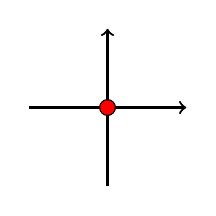
\begin{tikzpicture}
					\draw[->,thick] (-1,0) -- (1,0);
					\draw[->,thick] (0,-1) -- (0,1);
					\draw[fill=red] (0,0) circle (0.1);
				\end{tikzpicture}
			\end{center}
			\item \itemEq{k=1,r=2:\left\lbrace x\in\real^2\mid \left( \frac{x_1}{a_1}\right)^2-\left( \frac{x_2}{a_2}\right)^2=0\right\rbrace\notag}
			\begin{center}
				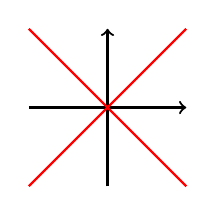
\begin{tikzpicture}
				\draw[->,thick] (-1,0) -- (1,0);
				\draw[->,thick] (0,-1) -- (0,1);
				\draw[thick, red] (-1,-1) -- (1,1);
				\draw[thick, red] (-1,1) -- (1,-1);
				\end{tikzpicture}
			\end{center}
			\item \itemEq{k=1,r=1:\left\lbrace x\in\real^2\mid \left( \frac{x_1}{a_1}\right)^2=0\right\rbrace\notag}
			\begin{center}
				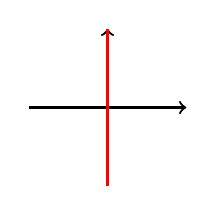
\begin{tikzpicture}
				\draw[->,thick] (-1,0) -- (1,0);
				\draw[->,thick] (0,-1) -- (0,1);
				\draw[thick, red] (0,-1) -- (0,1);
				\end{tikzpicture}
			\end{center}
		\end{itemize}
		\item \begin{itemize}
			\item\itemEq{k=2,r=2:\left\lbrace x\in\real^2\mid \left( \frac{x_1}{a_1}\right)^2+\left( \frac{x_2}{a_2}\right)^2=1 \right\rbrace\notag}
			\begin{center}
				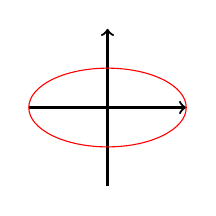
\begin{tikzpicture}
					\draw[->,thick] (-1,0) -- (1,0);
					\draw[->,thick] (0,-1) -- (0,1);
					\draw[red] (0,0) ellipse (1cm and 0.5cm);
				\end{tikzpicture}
			\end{center}
			\item\itemEq{k=1,r=2:\left\lbrace x\in\real^2\mid \left( \frac{x_1}{a_1}\right)^2-\left( \frac{x_2}{a_2}\right)^2=1 \right\rbrace\notag}
			\begin{center}
				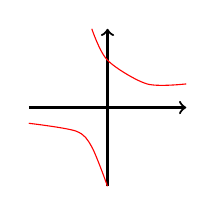
\begin{tikzpicture}
					\draw[->,thick] (-1,0) -- (1,0);
					\draw[->,thick] (0,-1) -- (0,1);
					\draw[red] plot [smooth] coordinates {(-0.2,1) (0,0.6) (0.5,0.3) (1,0.3)};
					\draw[red] plot [smooth] coordinates {(-1,-0.2) (-0.4,-0.3) (-0.2,-0.5) (0,-1)};
				\end{tikzpicture}
			\end{center}
			\item\itemEq{k=1,r=1:\left\lbrace x\in\real^2\mid \left( \frac{x_1}{a_1}\right)^2=1 \right\rbrace\notag}
			\begin{center}
				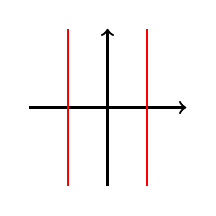
\begin{tikzpicture}
				\draw[->,thick] (-1,0) -- (1,0);
				\draw[->,thick] (0,-1) -- (0,1);
				\draw[thick, red] (-0.5,-1) -- (-0.5,1);
				\draw[thick, red] (0.5,-1) -- (0.5,1);
				\end{tikzpicture}
			\end{center}
			\item\itemEq{k=0,r=2:\left\lbrace x\in\real^2\mid -\left( \frac{x_1}{a_1}\right)^2-\left( \frac{x_2}{a_2}\right)^2=1 \right\rbrace=\emptyset\notag}
			\item\itemEq{k=0,r=1:\left\lbrace x\in\real^2\mid -\left( \frac{x_1}{a_1}\right)^2-\left( \frac{x_2}{a_2}\right)^2=1 \right\rbrace=\emptyset\notag}
		\end{itemize}
		\item \begin{itemize}
			\item\itemEq{k=1,r=1:\left\lbrace x\in\real^2\mid \left( \frac{x_1}{a_1}\right)^2-2x_2=0 \right\rbrace \notag}
			\begin{center}
				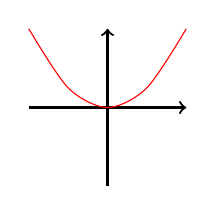
\begin{tikzpicture}
					\draw[->,thick] (-1,0) -- (1,0);
					\draw[->,thick] (0,-1) -- (0,1);
					\draw[red] plot [smooth] coordinates {(-1,1) (-0.5,0.25) (0,0) (0.5,0.25) (1,1)};
				\end{tikzpicture}
			\end{center}
		\end{itemize}
	\end{itemize}
\end{example}

\begin{remark}
	\begin{itemize}
		\item Ist $Q\subseteq\real^2$ eine Quadrik, $U\subseteq V$ affiner Untervektorraum, so ist $Q\cap U$ eine Quadrik in dem Sinne, dass $\exists f\text{ Isometrie}: f(U)=\real^k$ und $f(Q\cap U)$ ist eine Quadrik.
		\item Ebene Quadriken sind im wesentlichen Kegelschnitte, $Q'=\{x\in\real^3\mid x_1^2+x_2^2=x_3^2\}$, außer 2c und 2d in \propref{6_8_example}
	\end{itemize}
\end{remark}

\begin{remark}
	Die Situation wird deutlich übersichtlicher, wenn man den affinen Raum $\real^n$ durch Hinzunahme von Punkten im Unendlichen zum \begriff{projektiven Raum} $\mathbb{P}^n(\real)$ vervollstädigt und den Abschluss der Quadriken darin betrachtet. Es stellt sich dann heraus, dass vom projektiven Standpunkt aus die meisten ebenen Quadriken ähnlich aussehen. (Siehe Vorlesung \textit{Elementare Algebraische Geometrie})
\end{remark}
